\chapter{Detalles de Implementación y Resultados}\label{chapter:implementation}

Para la validación de la propuesta planteada a partir del esquema general de definición de los datos de entrada se concibió 
un prototipo de sistema. Este implementa los modelos de generación para el fútbol y el boxeo y permite la interacción
 con los mismos. Para facilitar la interacción se implementó a su vez una interfaz gráfica sencilla. A continuación se presentan 
 detalles generales del sistema, funciones de interés y una presentación de la interfaz creada. Finalmente se muestra el resultado del 
 texto producido por los modelos implementados. Se utilizó \emph{python} como 
 lenguaje de programación.
 
\section{Detalles generales del sistema}

\begin{figure}[!]
    \begin{center}
        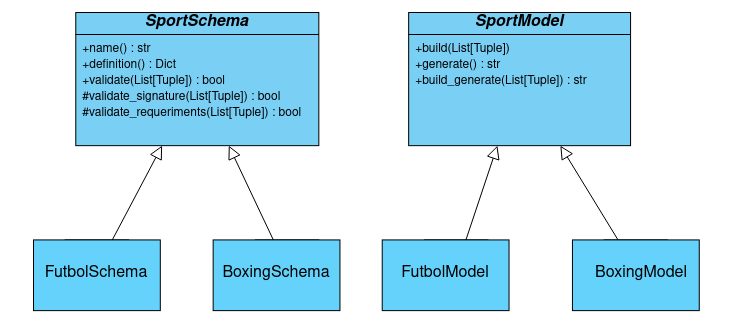
\includegraphics[width=\textwidth]{Graphics/classDef3.png}
    \end{center}
    \caption{Definición de las clases principales}
    \label{fig_classDef}
\end{figure}

Para la representación de los esquemas y de los modelos se crearon dos clases abstractas, \textit{SportSchema} y 
\textit{SportModel}. En la figura (\ref{fig_classDef}) se representan cada una con la signatura principal. 

Los esquemas, con el m\'etodo \emph{validate\_signature}, validan la entrada en cuanto a su signatura, o sea, comprueban que 
su representación en cada uno de los valores se corresponda con la definición. La \textit{definición} (m\'etodo \emph{definition}) 
de un esquema es el conjunto de valores admitidos por cada tipo principal (los tipos principales son los definidos en el 
meta esquema general). A su vez, el método \emph{validate\_requeriments} se utiliza para validar si en el conjunto de entrada
 existe un conjunto minimal de los datos a partir de los cuales es posible la generación de texto. El m\'etodo \emph{name} devuelve 
 un nombre identificativo del esquema, que debe ser único. La funcionalidad de \emph{validate} es una conjunción de los otros dos 
 métodos de validación. 




Los modelos para su correcto funcionamiento dependen de un primer llamado al método \emph{build} previo a cualquier 
secuencia de \emph{generate}. El método \emph{build} de los modelos es el que se encarga de procesar la entrada, hacer las 
transformaciones correspondientes de los datos. Durante su ejecución, los modelos completan toda la información 
necesaria para las distintas etapas de generación del texto que se definan. Para esto, se definen estructuras propias de cada 
modelo para representar la información. Con el uso de la información estructurada e interpretada en la construcción del modelo, 
con el método \emph{generate} se generan las distintas piezas textuales que conforman el reporte. El m\'etodo \emph{build\_generate} 
unifica un llamado a \emph{build} seguido de uno a \emph{generate}.

%Los modelos en build tienen que hacer todo el proceso de procesamiento de los datos, llenando tomados
%las variables y estructuras que son necesarias para generar el texto en cada una de las etapas. Luego
%en generate los modelos van en base a la representación interna de los datos, generando el texto de 
%caa una de las piezas comunicativas.

\begin{figure}[!]
    \begin{center}
        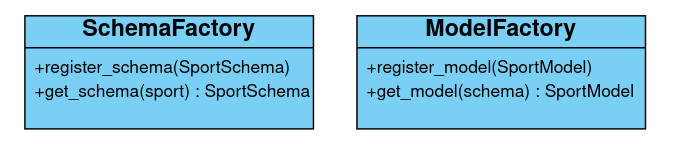
\includegraphics[width=\textwidth]{Graphics/factories.png}
    \end{center}
    \caption{Definición de las clases \emph{Factory}}
    \label{fig_classFactory}
\end{figure}


El flujo principal del programa se encuentra representado en el \textit{Algoritmo Principal} a continuación. Se utilizó el patrón 
\emph{Factory} (de Factoría, en español) para la selección de los modelos y los esquemas (Ver fig\ref{fig_classFactory}). 
Se planteó de esta forma, ya que el prototipo podría adaptarse más fácilmente a nuevos modelos y esquemas sin necesidad de grandes 
cambios en el código. %Las clases \textit{SchemaFactory} y \textit{ModelFactory}

\pagebreak

\begin{verbatim}
Algoritmo principal

  Entrada: knowdlage_tuple:List[Tuple], selected_sport
  Salida : str

    schema = schema_factory.get_schema(selected_sport)
    if not schema.validate(knowdlage_tuple):
        mostrar error
        FIN
    model = model_factory.get_model(schema)
    summary = model.build_generate(knowdlage_tuple)
    return summary

\end{verbatim}



\subsection{Proceso de realización. Selección de plantillas}

   El proceso de realización lingüística se lleva a cabo utilizando un conjunto de funciones que permiten la expresión correcta de la información 
en forma de oraciones. Para la representación de los datos los modelos consumen un sistema de plantillas hechas a mano. Un ejemplo de plantilla:

	\begin{center}
		\textit{$<$ portero $>$ atajó un penal a $<$ lanzador $>$ en el minuto $<$ minuto $>$}
	\end{center}

Las expresiones entre $<$ $>$ son las ranuras de las plantillas y se completan utilizando la información procesada de la entrada. Para facilitar la interpretación, 
a la expresión contenida entre $<$ \textit{clave} $>$ se le denominará clave de ranura.

  El proceso de selección y llenado de las plantillas se realiza a través de la función \emph{select\_template} (Algoritmo de selección de plantilla). 
  Esta recibe como parámetros el conjunto de posibles plantillas a emplear, el género a realizar, así como un diccionario de representación de la 
información donde las llaves coinciden con las posibles claves de ranura de las plantillas y los valores son los datos reales. 


  Como el sistema presenta cierto grado de sensibilidad ante la ausencia de algunos datos, es posible que haya plantillas para las que alguna ranura no tenga un 
valor real. La función \emph{\_is\_valid\_template} se utiliza para comprobar esto. El algoritmo selecciona aleatoriamente una plantilla del conjunto; si es válida, 
se selecciona, y si no, se descarta y se repite el proceso. Siempre se garantiza que habrá al menos una plantilla que sea funcional, ya que presentará las ranuras 
correspondientes al subconjunto minimal que admite el sistema en ese contexto. Para comprobar la validez de la plantilla primero 
se detectan las ranuras presentes en esta, utilizando la siguiente expresión regular: \textit{(r'$<$ (?P$<$key$>$[a-zA-ZáéíóúÁÉÍÓÚ\_]*) $>$')}.
  
\begin{verbatim}
Algoritmo de selección de plantilla
    
  Entrada: template_group:List[str], data_values:Dict[str,str], 
           genre:Genre.M | Genre.F
  Salida: str
    
    while not valid templat selected:
        template_selected = choice(tempalte_group)
        slots_values = []
        slots = slot_reggex.findall(template_group)
        for slot_value in slots:
            slots_values.append(slot_value)
        if __is_valid_template(slots_values, data_values):
            filled_template = fill_template(template_selected, 
                                slots_values, data_values)
            return disambiguate_template(filled_template, gender)
    return
    
\end{verbatim}   


  El método \emph{fill\_template} sustituye las ranuras de la plantilla por su valor real. Luego se pasa a desambiguar los términos de género. Como el sistema es 
adaptable tanto a la modalidad femenina como masculina de los deportes, es necesario realizar las expresiones en el género correcto. Las ranuras de género están 
presentes en algunas plantillas y tienen esta estructura: \$ \textit{clave} \$. Estas ranuras se detectan igualmente utilizando una expresión regular similar a la vista 
para las ranuras comunes. El caracter “@” también se utiliza dentro de las plantillas para hacer distinciones de género. Este proceso se produce en la 
función \emph{disambiguate\_template}.\\

\textbf{Funciones lingüísticas}\\

    Otras funciones se utilizan para mejorar el carácter léxico gramatical de las oraciones producidas. La función \emph{ordinal} transforma expresiones numéricas 
en su expresión ordinal (primer, segundo,  tercer, ..., vigésimo). La función \emph{numeral} transforma un valor numérico en su expresión léxica (uno, dos, tres). Esta 
abarca los números desde el 1 al 20 y los múltiplos de 10 hasta 100. Una vez que todas las transformaciones sobre las plantillas han sido realizadas, la función 
\emph{sentence\_lexical\_realization}, se utiliza para eliminar posibles errores, como espacios dobles, repetición de artículos (“el EL”), o corrige errores 
transformando expresiones como “de el” en su forma correcta “del”.\\


\textbf{Generación de expresiones de referencia}\\

    La generación se expresiones de referencia llevada a cabo se realiza a partir de los nombres propios de los individuos. Se utiliza la clase 
\emph{ReferentialExpressionGenerator} que se instancia con la lista de todos los nombres presentes. A partir de estos, utilizando el paquete de \textit{python}, 
\emph{nameparser} \brackcite{gulbranson}, se separa el nombre completo, en caso de que se brinde, en nombre y apellidos. Luego se determina qué referencias son ambiguas 
y se descartan. Cada vez que se solicite referencias a un nombre específico, el generador determina si esta es una primera referencia o una referencia tardía. Para 
las primeras referencias se emplea el nombre completo mientras que para segundas y terceras referencias se emplean los apellidos. En caso de muchas referencias a una 
misma persona, el generador podría utilizar el nombre si este no genera ambigüedad.


\section{Interfaz gráfica}

Para poder interactuar más fácil con la propuesta, se proporcionó una interfaz gráfica. Esta interfaz es sencilla
y se concibió utilizando el \emph{framework} de \textit{python streamlit}. Se da la opción a los usuarios de aportar
 datos en forma de archivos, ya sea a partir de definir la ruta local o cargando directamente el archivo.

 Para permitir  esta interacción se concibió una estructura intermedia para poder representar las tuplas 
de entrada en archivos \textit{.json} (ver fig\ref{fig_jsonexample}). Cada tupla se representa con las llaves: “1”, “2”,“3”,“4”
donde cada valor correspondiente representa el valor de la tupla en esa posición. Si no se proporciona uno de los 
valores, esa posición se considera vacía.

    \begin{figure}[!]
        \begin{center}
            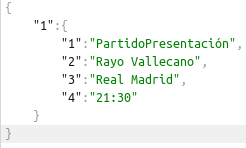
\includegraphics[scale=0.6]{Graphics/jsonexample.png}
        \end{center}
        \caption{Ejemplo de representación intermedia de una tupla de entrada en formato \textit{json}}
        \label{fig_jsonexample}
    \end{figure}

 Desde la primera interfaz se puede interactuar con el conjunto de datos de prueba que se concibieron
junto a la propuesta. Para ello hay que seleccionar el deporte deseado y uno entre los eventos de prueba.
El sistema mostrará el texto producido en pantalla, luego de presionar el botón “generar”.



\begin{figure}[!]
    \begin{center}
        
\includegraphics[width=\textwidth]{Graphics/GRED.png}
    \end{center}
    \caption{Interfaz del sistema}
    \label{fig_interfaz}
\end{figure}

\section{Resultados de la generación de texto}

    Para la validación de la propuesta se concibieron los modelos de fútbol y boxeo. Ambos debían, en base a su diseño 
generar resúmenes del evento a describir a partir de las tuplas de conocimiento del mismo. El texto debía mostrar cierto grado 
de variabilidad en la salida. O sea, distintos textos ante la misma instancia de datos. A continuación se muestran resultados de 
ambos modelos.\\

    \textbf{Fútbol}\\

  A continuación se muestran  dos variantes distintas producidas por el modelo para un mismo partido cuyo resultado reflejado por el 
\textit{Diario AS} se puede ver en figura \ref{fig_rayomadrid}. Un extracto de las tuplas que conforman la entrada se presenta en la 
figura \ref{fig_entradafutbol}.

\begin{figure}[!]
    \begin{center}
        
\includegraphics[scale=0.4]{Graphics/rayomadrid.png}
    \end{center}
    \caption{Muestra del resultado del partido y los goles por el \textit{Diario AS}}
    \label{fig_rayomadrid}
\end{figure}

\begin{figure}[!]
    \begin{center}
        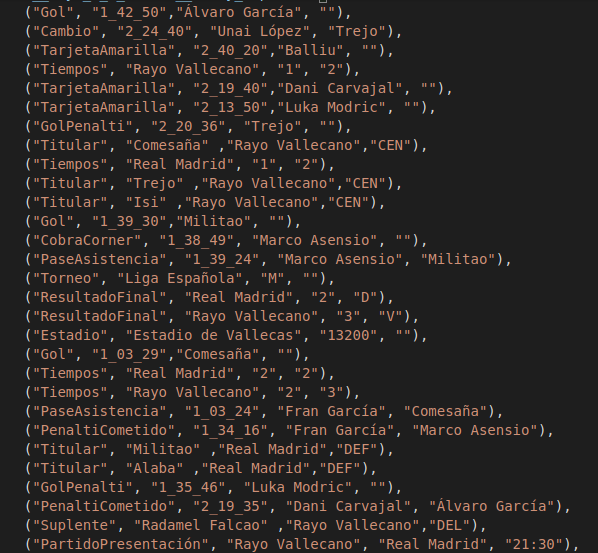
\includegraphics[scale=0.4]{Graphics/entradafutbol.png}
    \end{center}
    \caption{Extracto de las tuplas de entrada para el ejemplo del fútbol}
    \label{fig_entradafutbol}
\end{figure}

\begin{itemize}
    \item \textit{En el Estadio de Vallecas con la presencia de 13200 espectadores, Rayo Vallecano logró la victoria sobre Real Madrid 3 a 2.
    Asistido por Fran García, un gol de Comesaña en el minuto cuatro deshizo el cero en el marcador adelantando a Rayo Vallecano. Luka Modric con un gol desde el punto de penal en el minuto 36 puso nuevamente las tablas. En el minuto cuarenta, un tiro preciso de Militao, a pase de Marco Asensio, dió la delantera en el marcador a Real Madrid. Cuando corría el minuto 43, un buen disparo de Álvaro García acabó con la ventaja de Real Madrid. En el minuto 66, con un gol de penal, Trejo puso a Rayo Vallecano en ventaja.
    Trejo, centrocampista de Rayo Vallecano, fue el mvp del partido con un gol.}
    \item \textit{Rayo Vallecano se llevó la victoria 3 a 2 frente a Real Madrid en el Estadio de Vallecas ante un público de 13200 espectadores.
    En el cuatro, Comesaña con un tiro preciso declinó la balanza inicial a favor de Rayo Vallecano, el pase fue de Fran García. Luka Modric niveló el encuentro con un tiro ajustado preciso desde el punto de penal cuando corría el minuto 36. Cuando el crono marcaba el minuto cuarenta, con un disparo ajustado a pase de su compañero Marco Asensio, Militao deshizo la igualdad en favor de Real Madrid. Cuando el crono marcaba el minuto 43 una buena definición de Álvaro García acabó con la ventaja de Real Madrid. Trejo deshizo la igualdad en favor de Rayo Vallecano en el 66 con un gol desde los once metros.
    Con una anotación, el centrocampista de Rayo Vallecano, Trejo, fue el jugador más destacado del partido.}
\end{itemize}

El modelo desarrollado es capaz de generar textos que siguen la estructura elegida y cumple con el objetivo de 
crear un reporte de un partido de fútbol partiendo de la base de ser independiente de la fuente de datos utilizada. 

\pagebreak

    \textbf{Boxeo}\\


%    El modelo es capaz de generar los reportes, basados en la estructura planteada con independencia de la fuente de datos. 
%Se logró definir un esquema para el boxeo basado en el esquema general planteado. De la misma forma, durante la construcción de juegos 
%de datos para probar la propuesta se detectó que no abundan los sitios que describen el boxeo en función de eventos detallados. No es 
%objetivo de este trabajo evaluar la capacidad de encontrar datos que puedan ser adecuados al esquema propuesto. Se entiende será parte de 
%futuros trabajos.

    Se presentan dos muestras de reportes generados para una pelea entre Brian Mendoza y Jeison Rosario. Los datos se construyeron con el 
visionado de un extracto de la pelea en \textit{youtube.com}. Un ejemplo de la entrada utilizada puede verse en la figura \ref{fig_entradaboxeo}.

    \begin{figure}[!]
        \begin{center}
            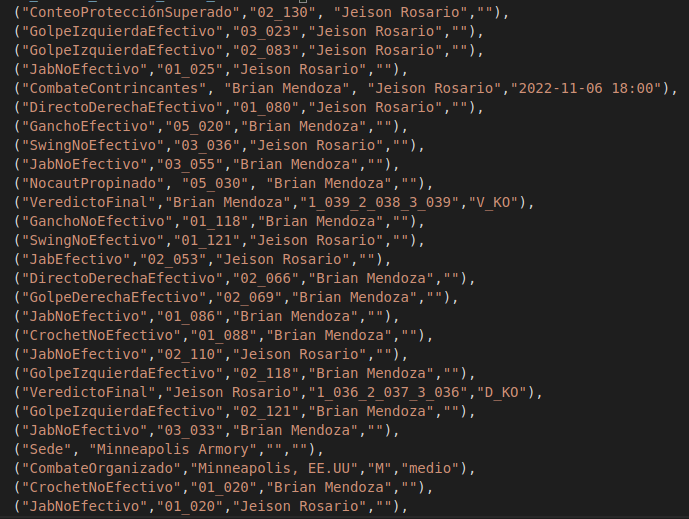
\includegraphics[scale=0.4]{Graphics/entradaboxeo.png}
        \end{center}
        \caption{Extracto de las tuplas de entrada para el ejemplo del boxeo}
        \label{fig_entradaboxeo}
    \end{figure}

    \begin{itemize}
        \item \textit{En el ring del Minneapolis Armory en la categoría de peso medio, con un imparable gancho Brian Mendoza obtuvo la victoria por nocaut frente 
        a Jeison Rosario en el quinto asalto.
        Mendoza hizo besar la lona a Rosario con un derechazo en el segundo asalto.}
        \item \textit{Ante los aficionados congregados en el Minneapolis Armory Brian Mendoza y Jeison Rosario cumplieron su cita en la categoría 
        de peso medio. Con un gancho Brian Mendoza obtuvo la victoria al noquear a Jeison Rosario en el quinto asalto.
        Mendoza puso en conteo de protección a Rosario con un inesperado puñetazo de derecha en el segundo asalto.}
    \end{itemize}

El modelo implementado fue capaz de generar textos que describían el combate de boxeo definido por los datos de entrada independiente de la fuente de obtención de los mismos. 
Mostró variabilidad, generando diferentes textos ante la misma entrada de datos. El texto generado respetó la estructura informativa definida.